\chapter{\label{ch2-mechanics}Camera Design \& Mechanics}

\minitoc

\notes[inline,caption={}]{
	\section{Plan}
	\subsection{Topics}
	\begin{itemize}
		\item Introduce TARGET architecture \& Wilkinson ADC
		\item Different TARGET versions
		\item FEE
		\item MAPMs
		\item SiPMS
		\begin{itemize}
			\item How they work
			\item Comparison investigations
			\item Property trade-offs
		\end{itemize}
		\item CHEC-M
		\item Changes for CHEC-S
		\item Future - MUSIC ASICs
	\end{itemize}
	\subsection{Questions}
	\begin{itemize}
		\item ?
	\end{itemize}
}

\section{Introduction}

\change[inline,caption={}]{
	\begin{itemize}
		\item number of pixels
        \item number of modules
        \item number of pixels per module
        \item number of cells
        \item pixel gaps
        \item module gaps
	\end{itemize}
}


\section{CHEC-M}

\change[inline]{schematic illustration of electronics}

\subsection{Multi-Anode Photomultiplier Tubes}

\change[inline]{connection between gain and hv}
\change[inline]{table of parameters}

\subsection{Front-End Electronics}

\subsubsection{Pre-Amplifiers}

\subsubsection{TARGET}

\begin{figure}
	\centering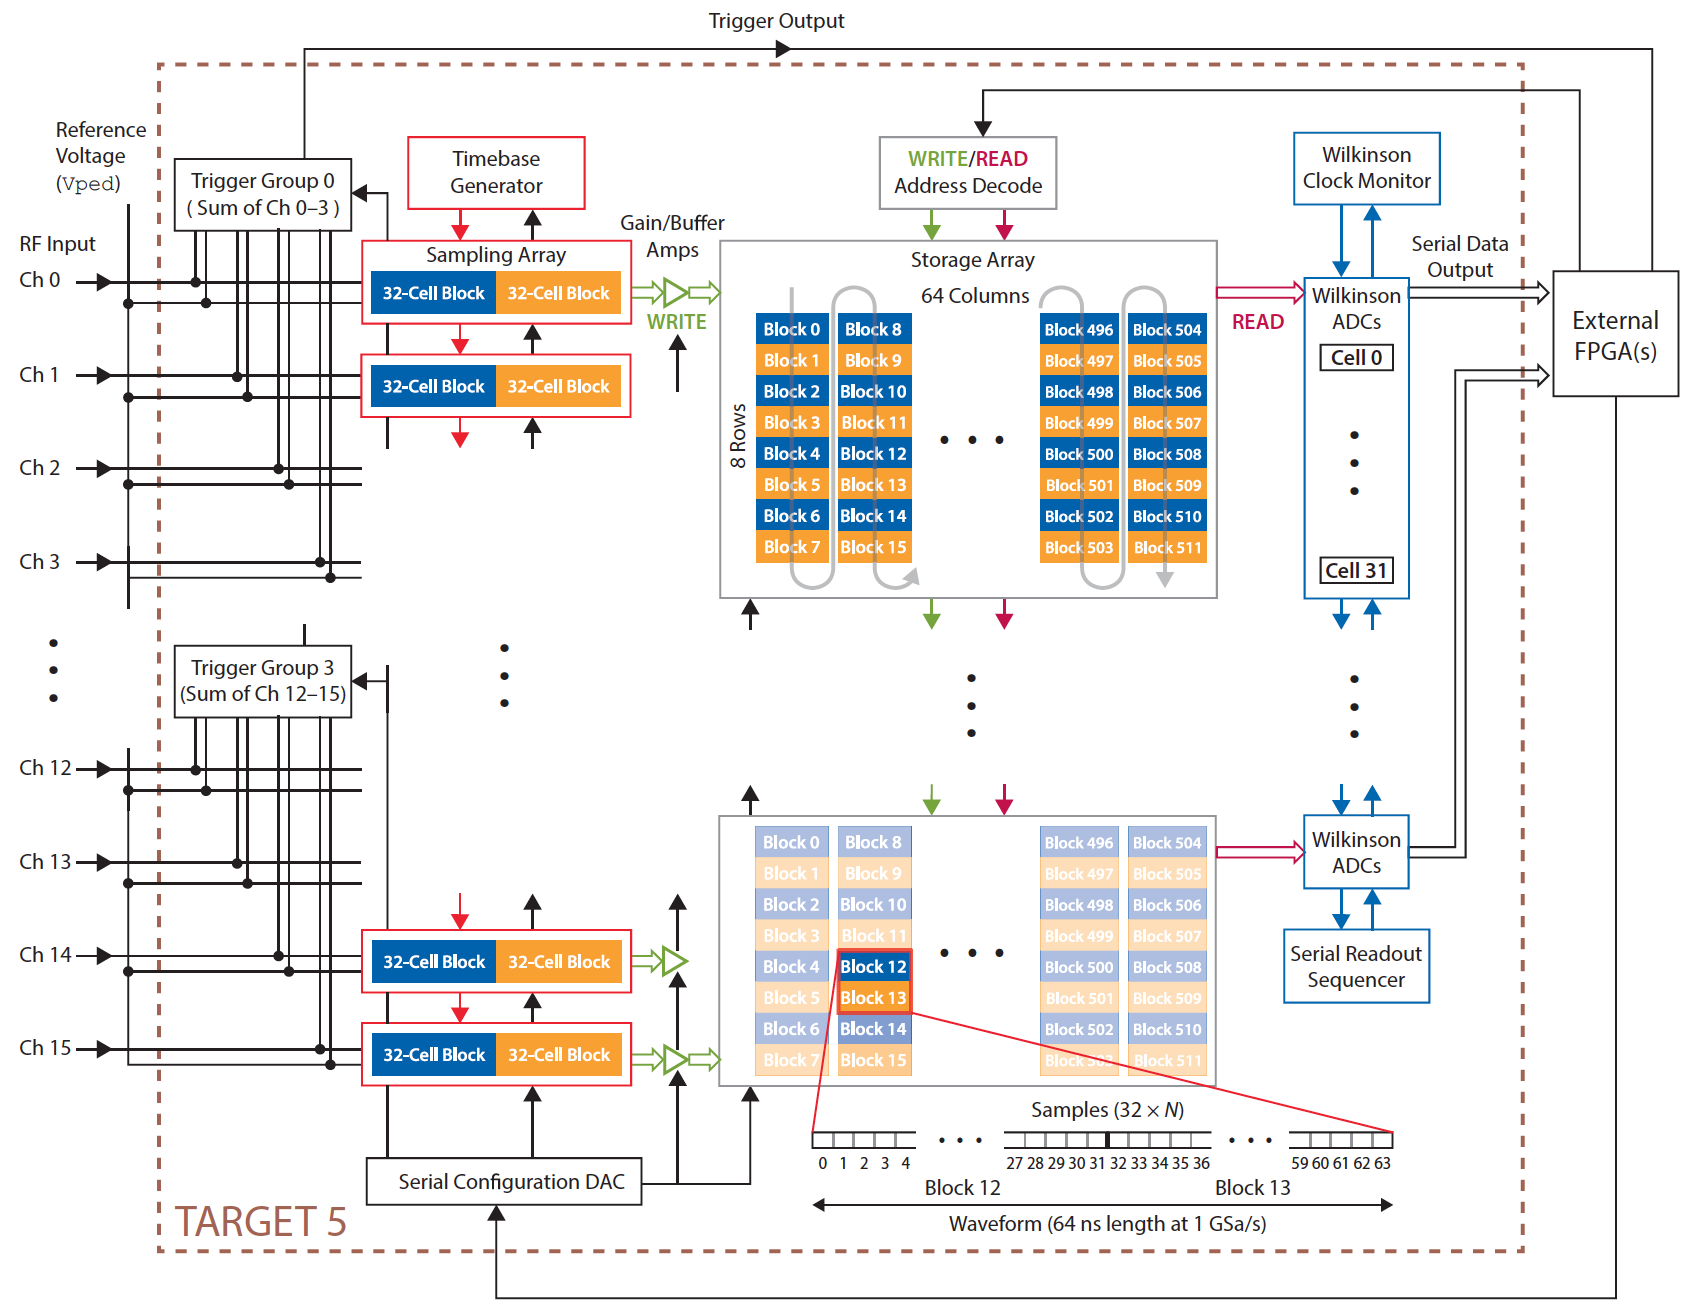
\includegraphics[width=\textwidth]{target5diagram} 
	\caption[Functional block diagram of the TARGET~5 ASIC.]{Functional block diagram of the TARGET~5 ASIC \cite{Albert2017} \change[inline]{Add more details}}
	\label{fig:target5diagram}
\end{figure}

\subsection{Back-End Electronics}

\subsubsection{Backplane}

\subsubsection{DACQ Boards}

\section{CHEC-S}

\subsection{Silicon Photomultipliers}

\change[inline]{connection between gain and bias voltage}
\change[inline]{table of parameters}

% \change[inline,caption={}]{
% 	\begin{itemize}
% 		\item V_b bias voltage
%         \item V_br breakdown voltage
%         \item V_over Overvoltage
%         \item PED does not change with temperature, but the breakdown voltage does, making it seem like the PDE changes
% 	\end{itemize}
% }

\subsection{TARGET-C}

\change[inline]{larger dynamic range, reference tf plot????}

\change{name of TARGET-C FPGA?}

\section{External Components} \label{section:external_components}

\subsection{LED Flashers} \label{section:led_flashers}

% Although not technically a part of the waveform processing chain, the LED flashers have an important role in the calibration system, especially for the final operation of the \gls{chec} cameras in \gls{cta}. Their purpose is to allow us to perform in situ calibration, by uniformly illuminating the camera via reflection in the secondary mirror. However, to achieve this, we must characterize and calibrate the LEDs such that we accurately know the illumination they are providing. \change[inline]{include some results on the LED calibration, and also mention their temperature dependence.}

\subsection{Chiller}

\section{Future}

\section{Laboratory Set-Up}

\section{Laboratory Calibration} \label{section:lab-calib}

In order to obtain reliable knowledge on the average illumination incident on the camera in our laboratory, it was necessary to calibrate the laser and filter wheel combination. This was of paramount importance for performing the camera flat-field calibration, and for obtaining a laboratory charge resolution result. There exists three stages required to achieve a calibration from filter-wheel position to average expected charge in each pixel:
\begin{enumerate}
\item Measuring the relationship between filter-wheel position and light transmissivity.
\item Measuring the relative amount of light each pixel receives due to its position on the focal surface.
\item Measuring an absolute illumination in photoelectrons for at least one filter-wheel position.
\end{enumerate}
Through combining the results of these stages, a conversion from filter-wheel position to expected number of photoelectrons in each pixel was obtained.

\subsection{Filter Wheel}

\begin{figure}
	\centering
    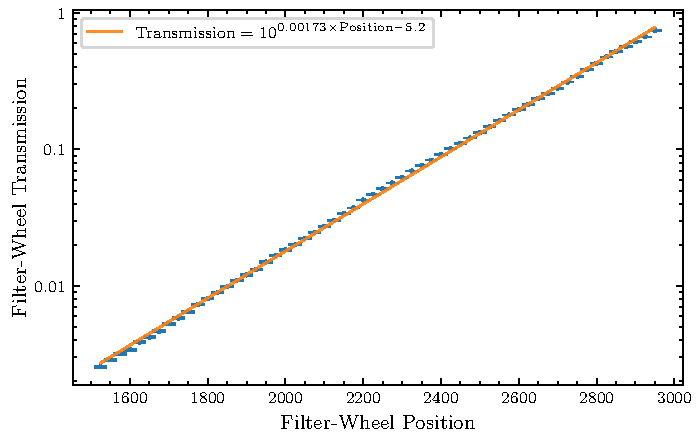
\includegraphics[width=\textwidth]{fw_position_justus} 
	\caption[Filter-wheel Position Calibration]{Logarithm of transmission versus position for the filter wheel. The relationship is fit with a straight line.}
	\label{fig:fw_position}
\end{figure}

\begin{figure}
	\centering
    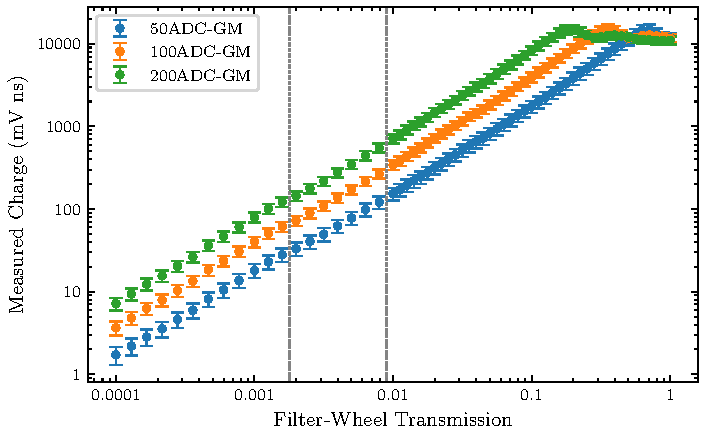
\includegraphics[width=\textwidth]{measured_versus_transmission} 
	\caption[Measured charge versus transmission]{Average charge across all CHEC-S pixels versus filter-wheel transmission. Three differently-gain-matched datasets are shown (50~ADC, 100~ADC, 200~ADC). Each gain matching results in a different bias voltage across the photosensor, and therefore a different gain, optical crosstalk, and PDE. Features shared between the datasets at a transmission value can only be due to errors in the filter-wheel calibration. Two clear features are highlighted by the vertical grey lines. Features shared at a measured charge value are due to shared properties in the Transfer Function (such as saturation).}
	\label{fig:measured_versus_transmission}
\end{figure}

\begin{figure}
	\centering
    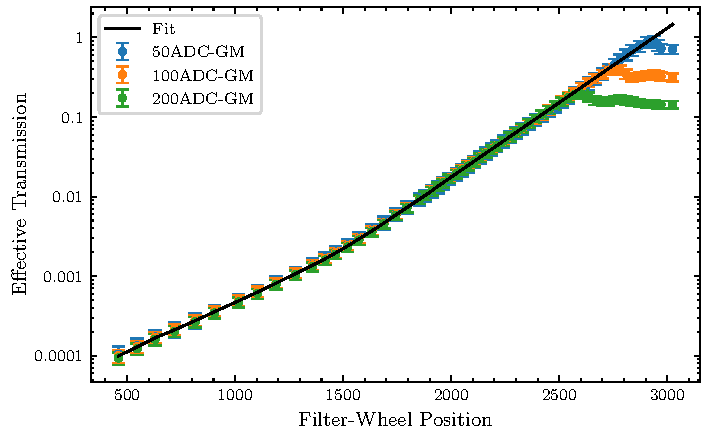
\includegraphics[width=\textwidth]{fw_correction} 
	\caption[Secondary filter-wheel calibration]{The measured charges from Figure~\ref{fig:measured_versus_transmission} converted into an ``effective transmission'', providing a filter-wheel calibration that is corrected for artefacts resulting from the first stage of calibration.}
	\label{fig:fw_correction}
\end{figure}

The calibration of the filter wheel was performed in two stages: an initial measurement with a reference \gls{sipmt} in order to obtain an approximate handle on the relative illumination, and a secondary correction using the camera at different gain settings.

\subsubsection{Reference SiPMT}

Using a single reference silicon photomultiplier pixel connected to an oscilloscope, centred on the camera focal plane, the ratio between the signal with and without the neutral-density filter was calculated for different filter-wheel positions (i.e. different attenuations). As the dynamic range of the reference \gls{sipmt} was limited, in order to cover the full range of filters attenuations, three approaches were utilised:
\begin{enumerate}
\item \textbf{Low-range} - Average illumination obtained from \gls{spe} spectrum, with a pre-amplifier attached to the \gls{sipmt}.
\item \textbf{Mid-range} - Average pulse area, with a pre-amplifier attached to the \gls{sipmt}.
\item \textbf{High-range} - Average pulse area, with no pre-amplifier attached.
\end{enumerate}
The overlapping values from each method were used to stitch the datasets together. The resulting points, shown in Figure~\ref{fig:fw_position}, were then used as a lookup table for the conversion from filter-wheel position to transmission.

\subsubsection{Camera Correction}

When looking at the average measured charge across the camera as a function of transmission, for three datasets where each has different bias voltages applied to the photosensors, features that share a position on the X axis can only occur from artefacts of the previous filter-wheel calibration. Figure~\ref{fig:measured_versus_transmission} indicates some of the artefacts which are easy to see. The measured charge was then converted into an ``effective transmission'' using the relation in Figure~\ref{fig:measured_versus_transmission}. By plotting the ``effective transmission'' against filter-wheel position, a new conversion from filter-wheel position to transmission was obtained from the fit shown in Figure~\ref{fig:fw_correction}.

\subsection{Illumination Profile} \label{section:illumination_profile}

Two contributions influence the relative amount of light each pixel receives, depending on its position on the camera focal surface. The first is due to the laser uniformity characteristics, the second is due to the curved focal surface of the camera.

\subsubsection{Laser Profile}

\begin{figure}
	\centering
    %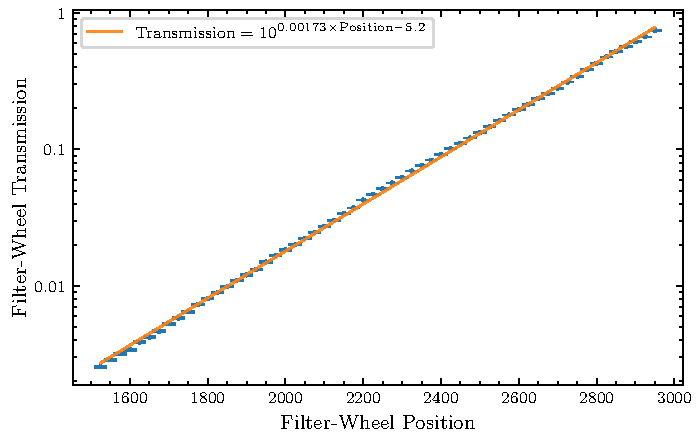
\includegraphics[width=\textwidth]{fw_position_justus} 
	\caption[Lab laser profile]{Spatial profile of the laser illumination along a flat plane in front of the camera, measured with a single reference \gls{sipmt} pixel attached to a robot arm. \change[inline]{Show value in each position, and then gradient fit?}.}
	\label{fig:light_profile}
\end{figure}

Despite attempts to homogenise the illumination from the laser-diffuser combination, there are still non-uniformities in the light received at the camera pixels that needed to be accounted for in the calibration. As shown in Figure~\ref{fig:light_profile}, a linear gradient in laser illumination exists across the x-y plane. This was found by attaching a single silicon photomultiplier pixel to a robot arm, and placing it at the camera position in from of the laser. Through the use of a single pixel, the amplitude measured is disentangled from the relative PDE. This pixel was then moved to each x-y position to calculate the ratio in signal amplitude, returning back to the origin to obtain a fresh value for comparison, thereby correcting for any deviations that may have occurred due to a change in temperature. The resulting distribution of ratios was fit with a linear gradient across the plane.

\subsubsection{Camera Geometry}

\begin{figure}
	\centering
    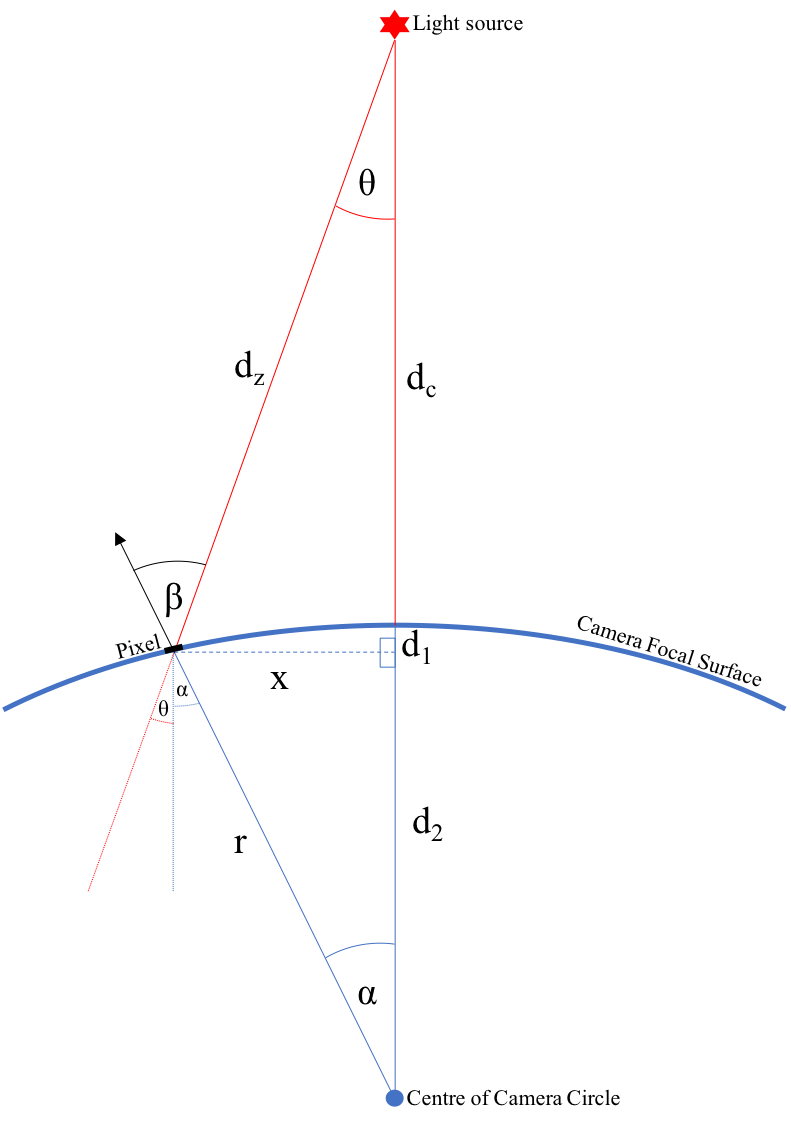
\includegraphics[width=0.75\textwidth]{laser_geometry} 
	\caption[Camera geometry correction schematic]{Two-dimensional geometry schematic of the laboratory set-up for uniform camera illumination, used to calculate the reduction in light level for each pixel depending on its distance from the camera centre.}
	\label{fig:laser_geometry}
\end{figure}

\change[inline]{Talk about how this is an approximation - modules are fixed along focal plane, light-source is somewhat between pointlike and at infinity, quote percentage that difference makes}

\change[inline]{Add not to scale on figure}

Due to the spherical camera focal surface, each pixel is at a different distance $d_z$ from the light-source, and therefore receives a different amount of light depending on its distance $x$ from the camera centre. Furthermore, at a ``viewing angle'' $\beta$, i.e. the angle between the normal to the pixel and the light-source, the amount of surface area of the pixel $A_P$ visible to the light-source is reduced. The visible surface area is known as the ``viewing area'' $A_V$. The combined geometric correction to the light intensity required to compensate for these effects is almost circularly symmetric, and therefore can be analytically approximated by using a two dimensional description of the camera, with a circular focal surface:

\begin{equation} \label{eq:geom_distance1}
d_1 = r - d_2 = r - \sqrt{r^2 - x^2},
\end{equation}
\begin{equation} \label{eq:geom_distance2}
d_z = \sqrt{x^2 + (d_c + d_1)^2} = \sqrt{x^2 + (d_c + r - \sqrt{r^2 - x^2})^2}.
\end{equation}
\begin{equation} \label{eq:viewing_area1}
\beta = \theta + \alpha = \sin^{-1}{\frac{x}{d_z}} + \sin^{-1}{\frac{x}{r}},
\end{equation}
\begin{equation} \label{eq:viewing_area2}
\frac{A_V}{A_P} = \cos{\beta},
\end{equation}
\begin{equation} \label{eq:geom_correction}
\frac{I_x}{I_c} = \frac{d_z^2}{d_c^2} \times \cos{\beta},
\end{equation}
where $A_P$ is the pixel area, $I_x$ is the intensity measured at the position of the pixel, $I_c$ is the intensity measured at the centre of the camera, and the remaining distances and angles are shown in Figure~\ref{fig:laser_geometry}.

The resulting geometry corrections to the intensity for each pixel, arising from Equation\ref{eq:geom_correction}, can be seen in Figure~\change{add figure}. 

The final illumination profile correction, combining both the laser profile and camera geometry, is shown in Figure~\change{add figure}. The description used for this calibration is only an approximation to the lab set-up. The following factors cause deviations from this model:
\begin{itemize}
\item The pixels are not precisely aligned on the spherical focal surface; the pixel angle is fixed to its module's angle. The modules are aligned on the spherical focal surface.
\item The light source is not point-like. It produces a diffuse emission, which likely reflects along the walls of the box.
\end{itemize}
A future study could further improve on the models used for the illumination correction.

\subsection{Absolute Illumination} \label{section:absolute_illumination}

\begin{figure}
	\centering
    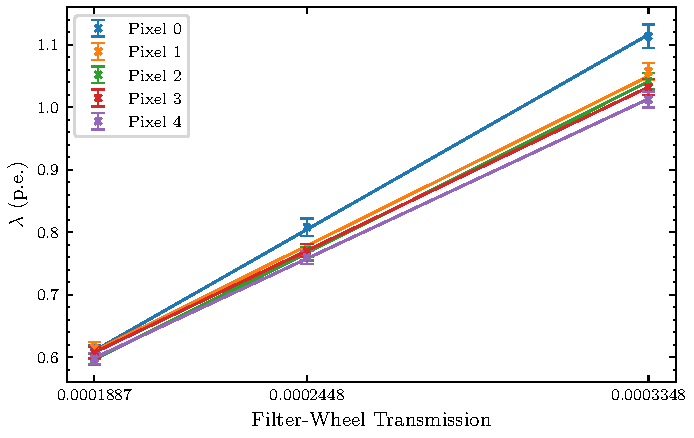
\includegraphics[width=\textwidth]{fw_calibration_fit} 
	\caption[Obtaining relationship between filter-wheel transmission and average illumination.]{Example of the linear regression to obtain the relationship between filter-wheel transmission and average illumination in photoelectrons ($\lambda$), for 5 pixels. The values of $\lambda$ are obtained from the simultaneous fits to the \gls{spe} spectra (Appendix~\ref{a1-spe}). The error bars on the points are the \si{1}{$\sigma$} parabolic errors obtained from the covariance matrix of the fit)}
	\label{fig:fw_calibration_fit}
\end{figure}

The method adopted to obtain a value for the absolute illumination was to use a fit to the \gls{spe} spectrum resulting from low-amplitude illumination of the pixels. Contained within this fit is the average illumination parameter, $\lambda$. The concept of the \gls{spe} fit is further covered in Chapter~\ref{ch5-calibration} and Appendix~\ref{a1-spe}.

By simultaneously fitting three illuminations, we obtained three values of $\lambda$ per pixel. With the three filter-wheel transmissions (corresponding to the three illuminations) on the x-axis, these values of $\lambda$ were linearly regressed (weighted by the \si{1}{$\sigma$} parabolic error of the fit, $\sigma_\lambda$) to obtain the gradient $M_\lambda$ and y-intercept $C_\lambda$ per pixel. This linear regression is shown in Figure~\ref{fig:fw_calibration_fit}. The y-intercept represents the value of $\lambda$ one would get with zero filter-wheel transmission, and therefore indicates the \gls{nsb} and \gls{dcr}. The variation in $M_\lambda$ across the pixels arises from the folding of the illumination profile and the relative \gls{pde}. Therefore, the next step was to correct for the illumination profile contribution to the gradient. The resulting spread of $M_\lambda$ is solely from the relative \gls{pde} (Figure~\change{add figure, in this chapter or results chapter?}). The calibration from filter-wheel transmission $T_\text{FW}$ to the average illumination across the whole camera $\average{I}_{pe}$ is then obtained by taking the averages of the linear regression coefficients:

\begin{equation} \label{eq:average_camera_illumination}
\average{I}_{pe} = \average{M}_\lambda T_\text{FW} + \average{C}_\lambda,
\end{equation}

\subsection{Average Expected Charge}

\begin{figure}
	\centering
    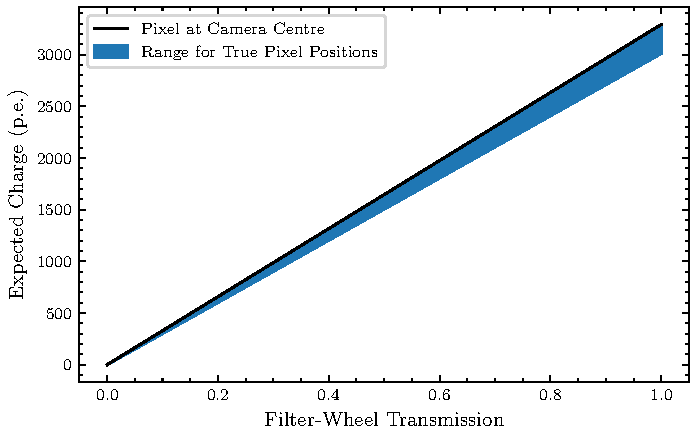
\includegraphics[width=\textwidth]{fw_calibration} 
	\caption[Calibration from filter-wheel transmission to expected charge]{Relationship between filter-wheel transmission and average expected charge in photoelectrons resulting from the filter-wheel calibration. The black line shows the conversion for a theoretical pixel positioned exactly at the camera centre. The error bars are calculated from the weighted standard deviation of the gradient estimates between the pixels, explained in Section~\ref{section:fwerr}}
	\label{fig:fw_calibration}
\end{figure}

As we corrected for the \gls{nsb} in the extracted signal value (Section~\ref{section:photosensor_calib}), the \gls{nsb} contribution to Equation~\ref{eq:average_camera_illumination} ($\average{C}_\lambda$) is subtracted to give us the charge we expect when illuminating the camera with a filter-wheel transmission $T_\text{FW}$, for a theoretical pixel perfectly positioned at the camera centre. This relation is shown in Figure~\ref{fig:fw_calibration}. To obtain the average expected charge $Q_\text{Exp}$ for each true camera pixel, this relation must be folded with the illumination profile correction factor $F_\text{pix}$:
\begin{equation} \label{eq:average_expected_charge}
Q_\text{Exp} = \average{M}_\lambda T_\text{FW}F_\text{pix}.
\end{equation}
This expression is important for the flat-fielding calibration (Chapter~\ref{ch5-calibration}) and the calculation of the \textit{Charge Resolution} for lab measurements (Chapter~\ref{ch7-performance}), as it tells us for a certain pixel and filter-wheel transmission, what charge we should expect to measure on average.

\subsection{Consideration of Errors and Uncertainty} \label{section:fwerr}

When performing the weighted linear regression between $\lambda_i$ and filter-wheel transmission $T_{FW_i}$ (with weights $w_i = \frac{1}{\sigma_{\lambda_i}^2}$ accounting for the parabolic error in $\lambda_i$), the standard error on the estimate of the gradient per pixel, $\sigma_{M_\lambda}$, can be calculated with the relation:
\begin{equation} \label{eq:merr}
\sigma_{M_\lambda} = \sigma_r \sqrt{\frac{\sum w_i}{\sum w_i \sum w_i T_{FW_i}^2 - (\sum w_i T_{FW_i})^2}},
\end{equation}
\begin{equation} \label{eq:reserr}
\sigma_r = \sqrt{\frac{\sum w_i (\lambda_i - \lambda_{r_i})^2}{N - 2}},
\end{equation}
where $\sigma_r$ is the mean square error of the regression, $N$ is the number of data points, and $\lambda_{r_i}$ is the regressed value at a transmission $T_i$. 

During the correction for the illumination profile on the gradient estimates, the illumination correction factors are also applied to the standard error on the gradient estimate.

While calculating the average gradient across the camera, $\average{M}_\lambda$, the individual gradient estimates are weighted by their corresponding standard error. To calculate an uncertainty on the resulting value for $\average{M}_\lambda$, the weighted standard deviation between the gradient estimates is also calculated. This uncertainty is illustrated in the error bars in Figure~\ref{fig:fw_calibration}. The resulting conversion value from filter wheel transmission to expected charge for a theoretical pixel located at the centre of the camera was calculated to be $\average{M}_\lambda = \SI[separate-uncertainty = true]{3192.93 \pm 254.07}{\pe}$.


\section{Readout Characteristics} \label{section:readout_characteristics}

\change{define ADC}

\change{monitoring information}

\section{Nomenclature}

\change[inline]{charge/signal, waveform/trace, events}